\section{Hinzufügen von Objekten zum Testszenario \dcsecondauthorshort}
\label{ssec:evaluation:messungen:objekte_hinzufuegen}
Im realen Straßenverkehr befinden sich in der Regel mehr Objekte im Sichtbereich des Fahrers bzw. der Kamera als die bis jetzt im Parcours alleinig vorhandenen Fahrbahnmarkierungen. Diese Gegenstände können für die Trajektorieplanung relevant sein (Hindernisse) oder in keinem Zusammenhang damit stehen (Objekte abseits der Straße). Da der bis jetzt implementierte Fahrspurverfolgungsalgorithmus keine Hinderniserkennung und -vermeidung besitzt, kann hier nur auf Gegenstände neben der Fahrspur eingegangen werden. In diesem Abschnitt sollen Untersuchungen stattfinden, ob die Erkennung des Straßenverlaufs auch bei Hinzufügen weiterer Gegenstände zum Testszenario noch zufriedenstellend abläuft.

\subsection{Betrachtungen zur Bildvorverarbeitung}
\label{par:evaluation:riverflow:messungen:objekte_hinzufuegen}
Vor der Durchführung von Testfahrten muss die Frage gestellt werden, wann dem Parcours hinzugefügte Elemente einen Einfluss auf die Fahrspurerkennung haben können. Da die Filterung und anschließende Binarisierung des entzerrten Graustufenbildes den Ausgangspunkt für darauffolgende Programmkomponenten darstellen, muss das Objekt die \glqq Hürde\grqq\ dieser Informationsreduktion überwinden können. Konkret bedeutet dies, dass sein Kontrast im Vergleich zum umliegenden Szenario groß genug sein muss, um als schwellwertüberschreitende Filterantwort des Kantendetektors im Binärbild aufzutreten oder als relevantes Maxima auf einer Scanline gefunden zu werden (s. Abschnitt \ref{sec:bildvorverarbeitung:binarisierung} bzw. \ref{ssec:fahrspurerkennung:kalman:messung}).
Als Vorversuch wurden farbige Blätter (Abb. \ref{fig:evaluation:riverflow:test_kontraste_roh}) verschiedener Helligkeit (Abb. \ref{fig:evaluation:riverflow:test_kontraste_entzerrt}) im Testszenario platziert. Abbildung \ref{fig:evaluation:riverflow:test_kontraste_gefiltert} zeigt wie erwartet, dass nur sehr dunkle Farben eine ausreichend große Filterantwort hervorrufen, welche im Binärbild (Abb. \ref{fig:evaluation:riverflow:test_kontraste_binarisiert}) als Kante vermerkt wird. Auffällig ist auch, dass die Eckpunkte der Blätter eine besonders große Filterantwort bewirken, die eigentlichen Kanten aber nur beim roten (teilweise) und schwarzen Blatt erkannt werden.

\begin{figure}[htbp] % [htb]
%\centering
%\hfill
\subfloat[roh\label{fig:evaluation:riverflow:test_kontraste_roh}]{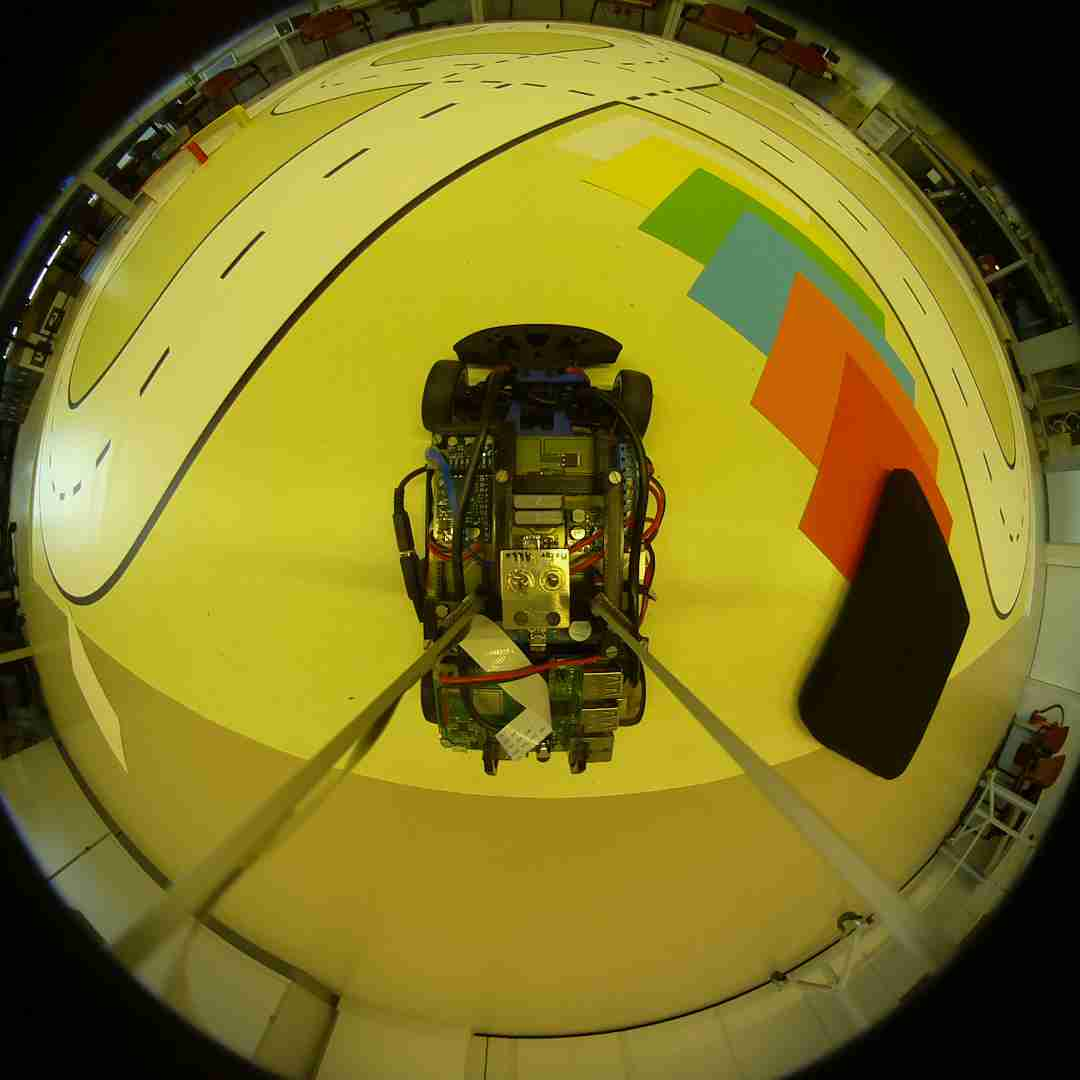
\includegraphics[width=0.49\textwidth]{evaluation_riverflow_test_kontraste_roh}}
\hfill
\subfloat[entzerrt\label{fig:evaluation:riverflow:test_kontraste_entzerrt}]{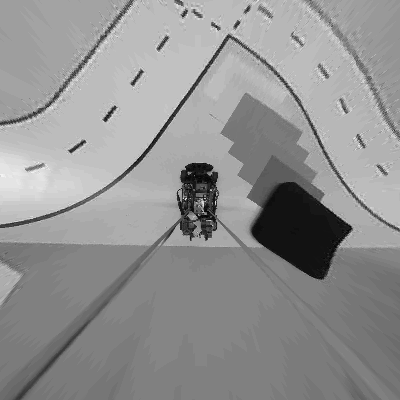
\includegraphics[width=0.49\textwidth]{evaluation_riverflow_test_kontraste_entzerrt}}
\hfill
\subfloat[gefiltert\label{fig:evaluation:riverflow:test_kontraste_gefiltert}]{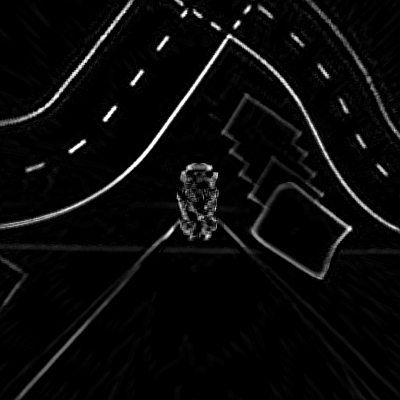
\includegraphics[width=0.49\textwidth]{evaluation_riverflow_test_kontraste_gefiltert}}
\hfill
\subfloat[binarisiert\label{fig:evaluation:riverflow:test_kontraste_binarisiert}]{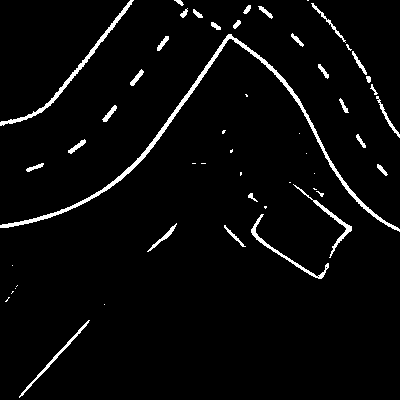
\includegraphics[width=0.49\textwidth]{evaluation_riverflow_test_kontraste_binarisiert}}
%\hfill
\label{fig:evaluation:riverflow:test_kontraste}
\caption{Vorversuch Kontraste zusätzlicher Objekte im Testszenario}
\end{figure}

\subsection{Objekte neben der Fahrspur}
Es wurden einige Quader, in den Farben des in Abschnitt \ref{par:evaluation:riverflow:messungen:objekte_hinzufuegen} untersuchten Papiers, im Parcours positioniert (s. Abb. \ref{fig:evaluation:riverflow:test_kontraste_versuchsaufbau_haeuser}). Hierbei wurde bei 3 Fahrten der Abstand zur seitlichen Fahrbahnmarkierung von \SI{16}{cm} (größer der Länge einer Scanline) über \SI{4}{cm} (kleiner der Länge einer Scanline) hin zu \SI{0}{cm} verändert.

Können die Scanlines die Kanten eines solchen Objektes nicht erreichen, so ist kein Einfluss auf die Erkennung der Randlinien zu erwarten. Ist der Kontrast eines Quaders zur hellgrünen Grundfarbe des Testszenarios zu gering, so ist eine Fehldetektion aufgrund dessen ebenfalls ausgeschlossen. Eventuelle Beeinträchtigungen des Riverflow-Algorithmus sind somit nur bei den Versuchen mit \SI{4}{cm} und \SI{0}{cm} Abstand bei dunklen Farben der \glqq Störobjekte \grqq\ zu erwarten.

Der Roboter fuhr jedoch auch in diesen Konstellationen fehlerfrei die Runde. Es konnten bei allen Testfahrten keine falsch in der Weltkarte eingetragenen Punkte identifiziert werden.
 
\begin{figure}[htbp] % [htb]
\centering
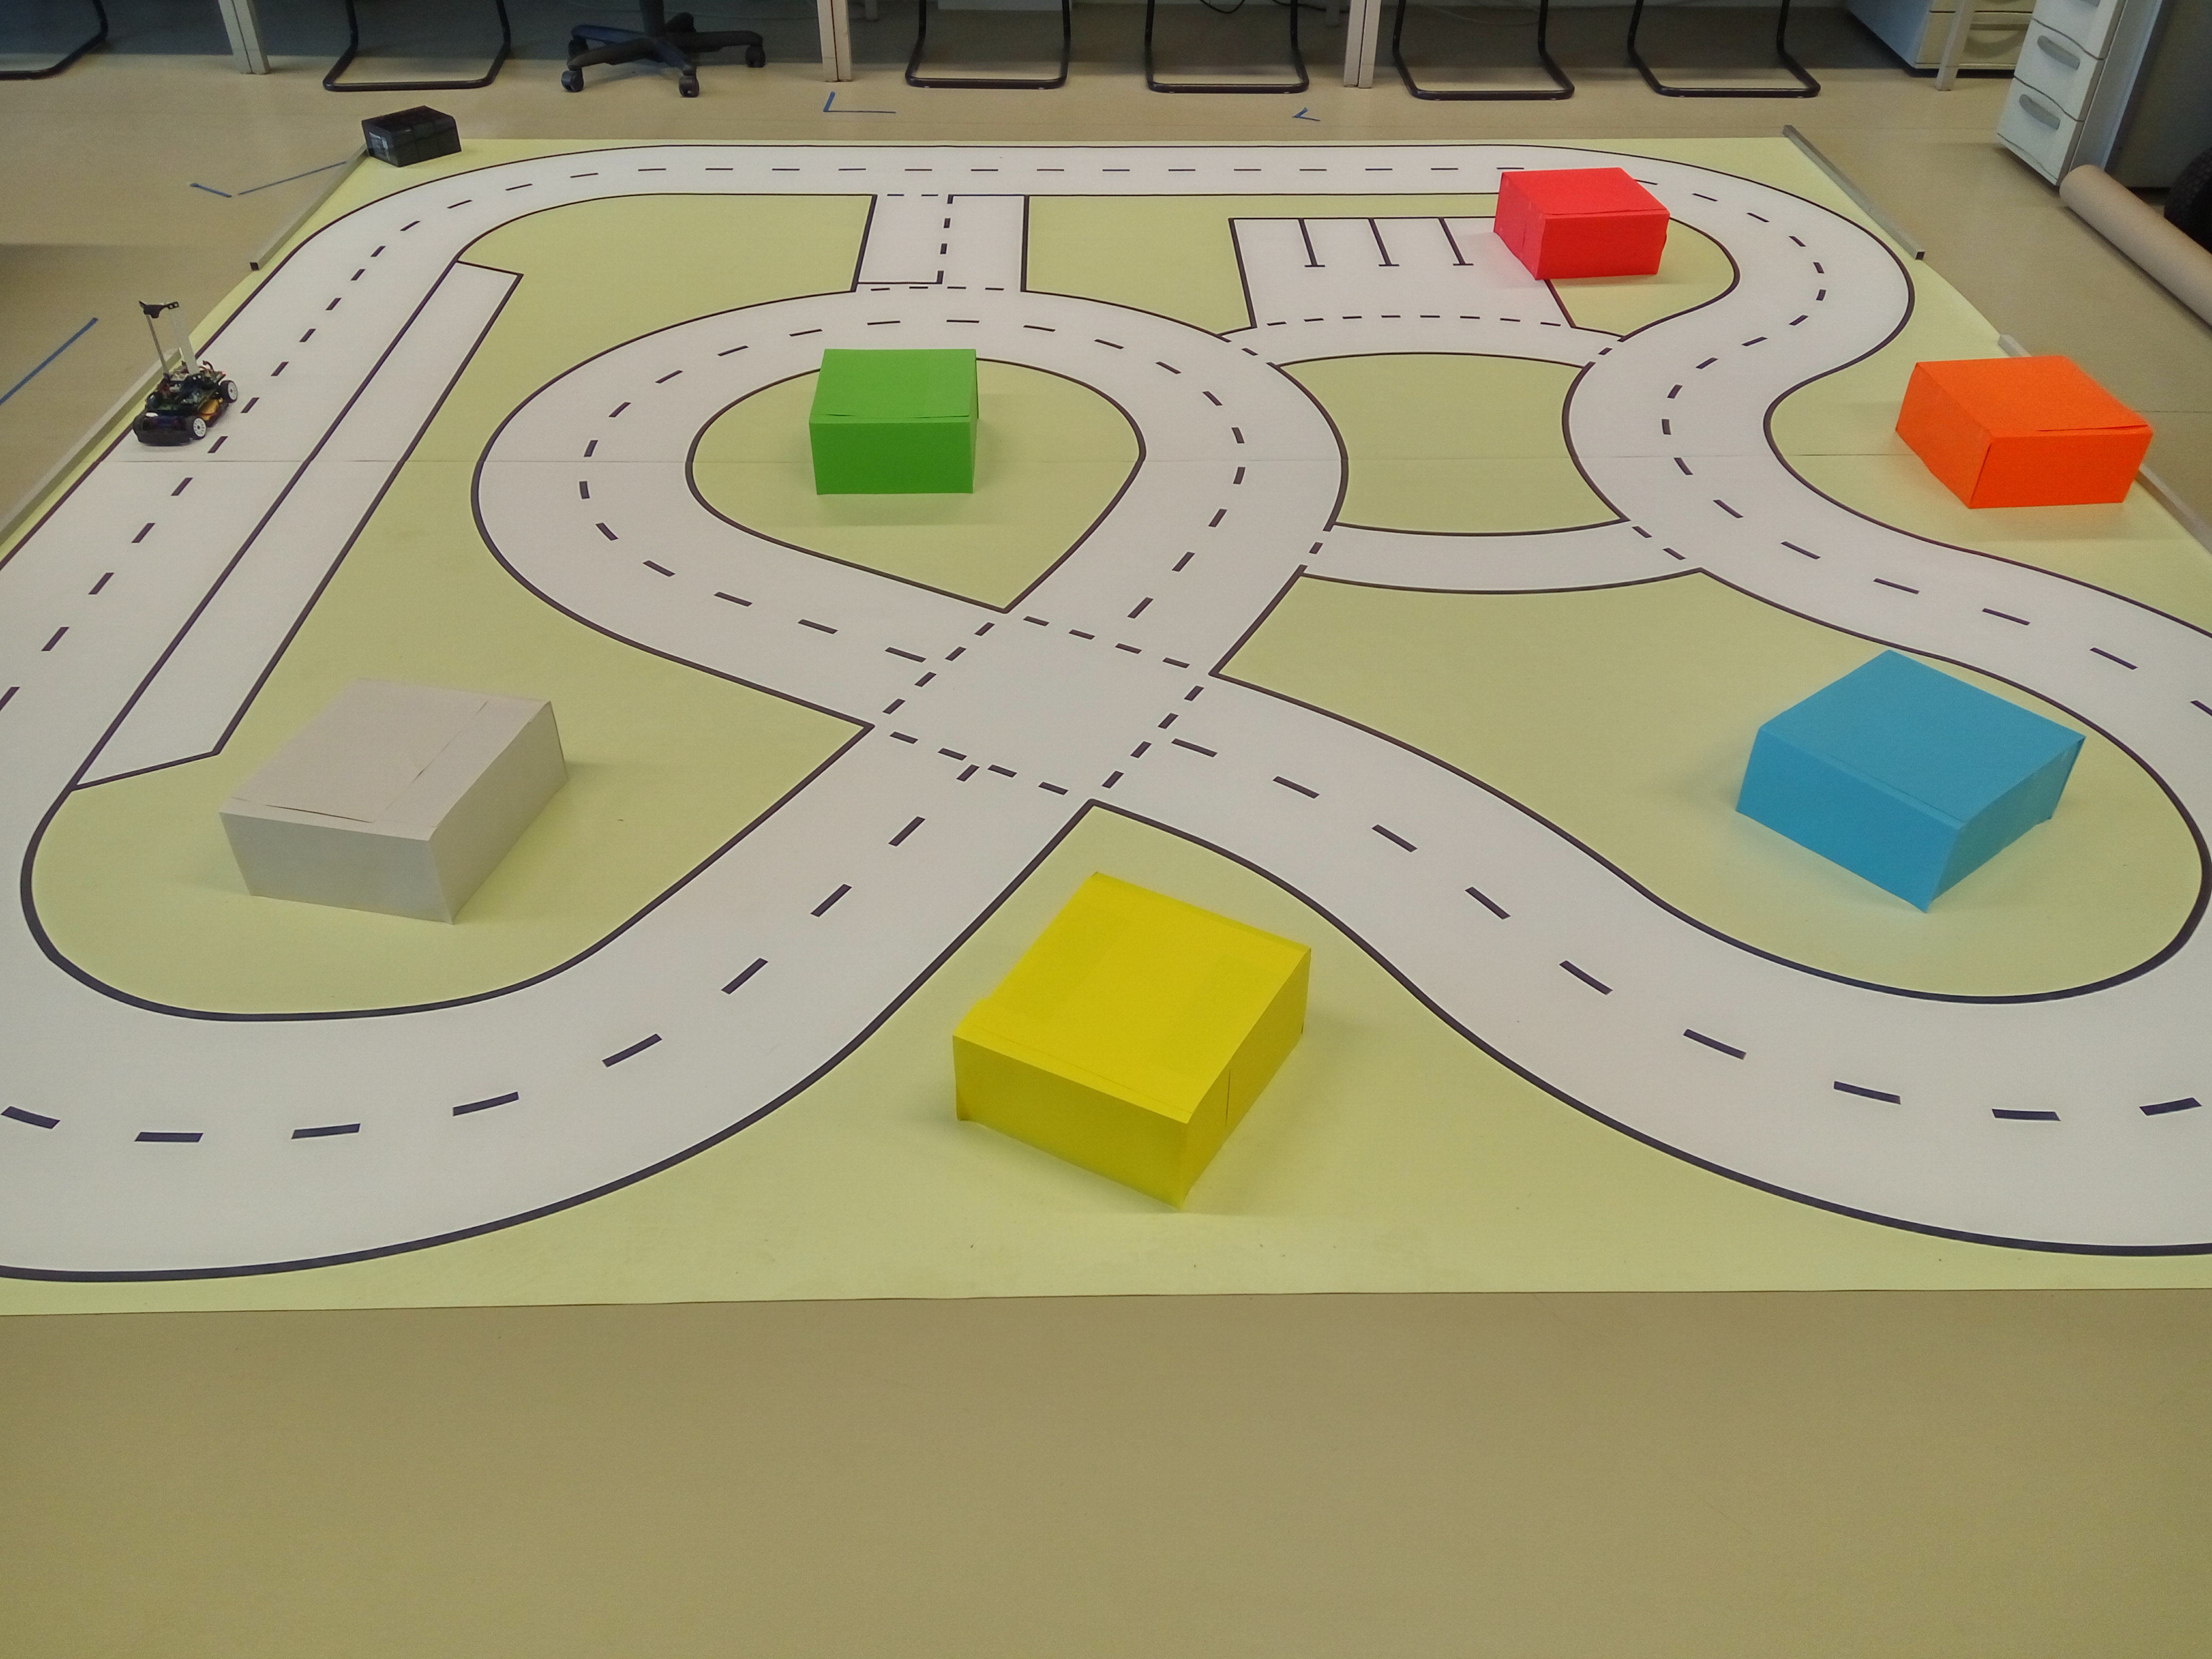
\includegraphics[width=0.5\textwidth]{evaluation_riverflow_test_kontraste_versuchsaufbau_haeuser}
\caption{Versuchsaufbau farbige Quader im Testszenario}
\label{fig:evaluation:riverflow:test_kontraste_versuchsaufbau_haeuser}
\end{figure}

Diese Robustheit gegenüber den hinzugefügten Quadern wurde auf die Verifikation der Punkte nach der Erkennung zurückgeführt, somit soll nun noch die Performanz des Algorithmus ohne diese Komponente betrachtet werden. Charakteristisch für eine Beeinträchtigung an dieser Stelle wäre das Anlegen vieler Hypothesen (möglicher Verläufe der Randlinien), da auf einer Scanline mehrere potentielle zentral auf einer Fahrbahnmarkierung gelegenen Punkte gefunden werden (s. Abschnitt \ref{sssec:fahrspurerkennung:riverflow:randlinie:zentraler_algorithmus}).
\begin{figure}[htbp] % [htb]
%\centering
%\hfill
\subfloat[keine \glqq Störobjekte\grqq \label{fig:evaluation:riverflow:hypos_hist_inf}]{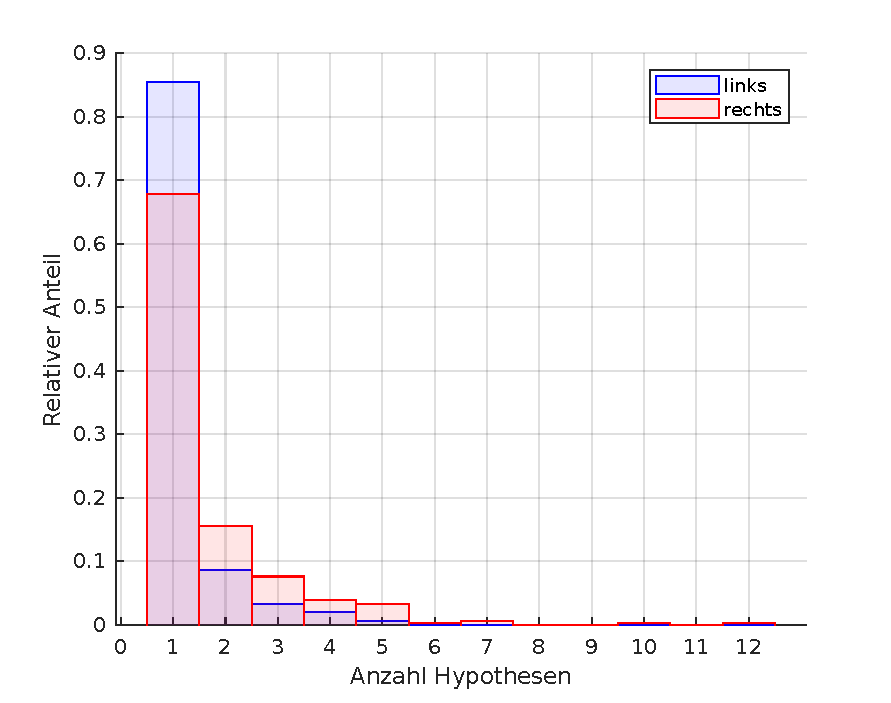
\includegraphics[scale=\mtlstscale]{evaluation_riverflow_hypos_hist_inf}}
\hfill
\subfloat[\SI{16}{cm}\label{fig:evaluation:riverflow:hypos_hist_16}]{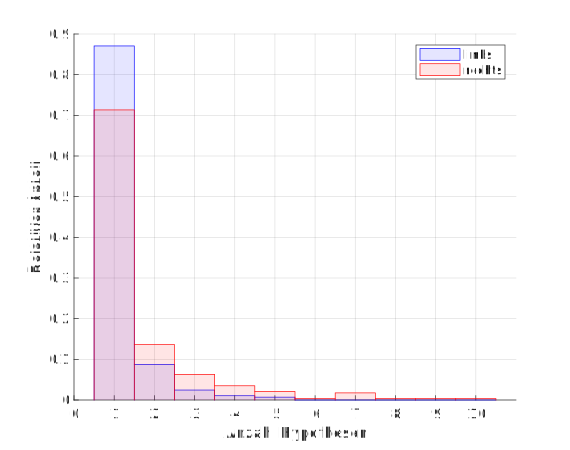
\includegraphics[scale=\mtlstscale]{evaluation_riverflow_hypos_hist_16}}
\hfill
\subfloat[\SI{4}{cm}\label{fig:evaluation:riverflow:hypos_hist_04}]{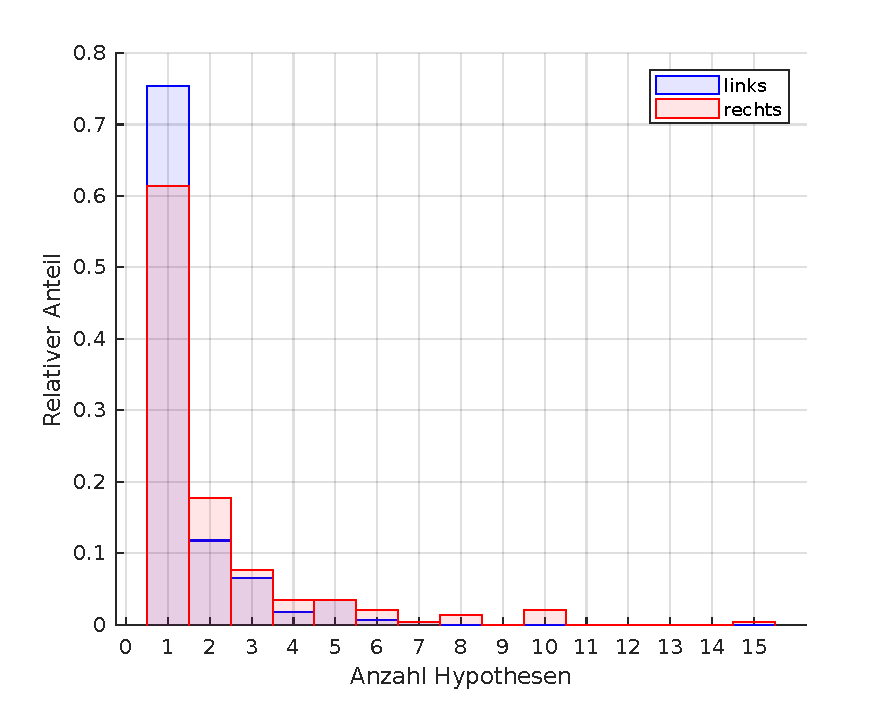
\includegraphics[scale=\mtlstscale]{evaluation_riverflow_hypos_hist_04}}
\hfill
\subfloat[\SI{0}{cm}\label{fig:evaluation:riverflow:hypos_hist_00}]{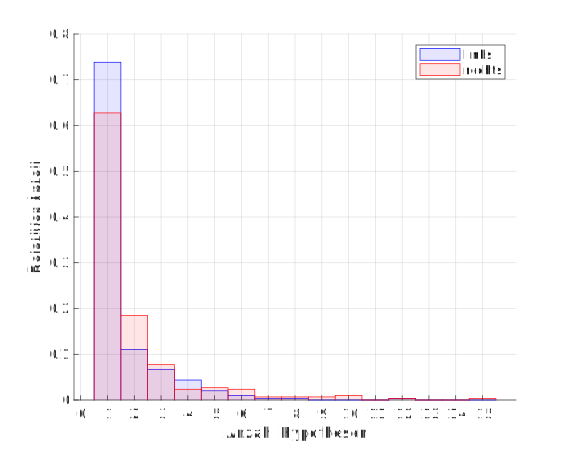
\includegraphics[scale=\mtlstscale]{evaluation_riverflow_hypos_hist_00}}
%\hfill
\caption{Histogramme Hypothesenanzahl mit \glqq Störobjekten\grqq\ im Testszenario; Variation des Abstandes von der Fahrspur}
\label{fig:evaluation:riverflow:hypos_hists}
\end{figure}

Abbildung \ref{fig:evaluation:riverflow:hypos_hists} bestätigt diese Vermutung, es ist ein häufigeres Auftreten mehrerer Hypothesen für die seitlichen Fahrbahnmarkierungen zu beobachten, wenn diese in die von den Scanlines aufgespannten \gls{acr:roi}'s platziert werden. Beispiele für diese Fehlerkennungen sind in Abbildung \ref{fig:evaluation:riverflow:hypos_riverflow_plots} zu sehen.
\begin{figure}[htbp] % [htb]
%\centering
%\hfill
\subfloat[\label{fig:evaluation:riverflow:hypos_riverflow_plot_1}]{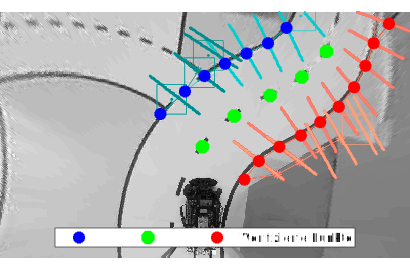
\includegraphics[width=0.49\textwidth]{evaluation_riverflow_hypos_riverflow_plot_1}}
\hfill
\subfloat[\label{fig:evaluation:riverflow:hypos_riverflow_plot_2}]{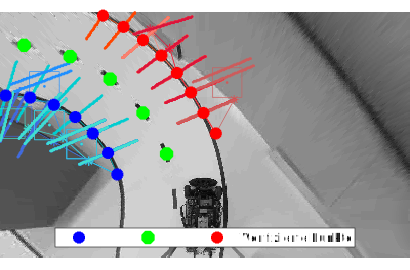
\includegraphics[width=0.49\textwidth]{evaluation_riverflow_hypos_riverflow_plot_2}}
\hfill
\subfloat[\label{fig:evaluation:riverflow:hypos_riverflow_plot_3}]{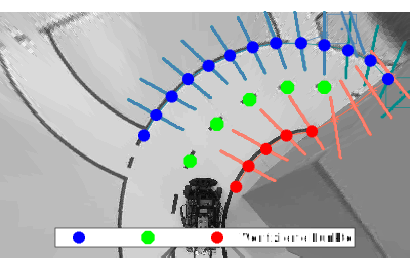
\includegraphics[width=0.49\textwidth]{evaluation_riverflow_hypos_riverflow_plot_3}}
\hfill
\subfloat[\label{fig:evaluation:riverflow:hypos_riverflow_plot_4}]{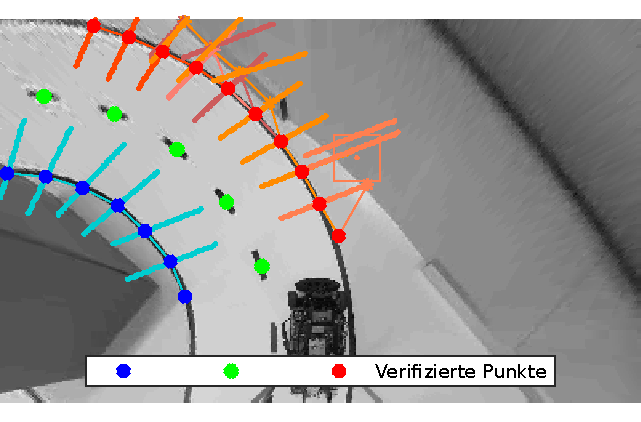
\includegraphics[width=0.49\textwidth]{evaluation_riverflow_hypos_riverflow_plot_4}}
%\hfill
\caption{Beispiele für die Erkennung mehrerer Hypothesen mit \glqq Störobjekten\grqq\ im Testszenario}
\label{fig:evaluation:riverflow:hypos_riverflow_plots}
\end{figure}

Ein weiterer Grund für die Detektion mehrerer möglicher Verläufe der Randlinie stellt, wie in Abbildung \ref{fig:evaluation:riverflow:hypos_riverflow_plot_4} zu sehen, die Erkennung schon immer im Testszenario vorhandener, bis jetzt nicht weiter berücksichtigter Kanten dar. Die Ränder der PVC-Plane, auf welche die Strecke gedruckt wurde oder die zum Beschweren dieser genutzten Alu-Profile sind häufig die Ursache solcher Fehldetektionen.

Die unter Nachteile in Abschnitt~\ref{sec:evaluation:riverflow:diskussion_prinzip} vermutete Verlängerung der Bearbeitungszeit konnte bestätigt werden, Abb. \ref{evaluation:riverflow:hypos:times_04} stellt den Zusammenhang zwischen der Anzahl verfolgter Hypothesen und der damit verbundenen Dauer der Detektion seitlicher Fahrbahnmarkierungen dar.

\begin{figure}[htbp] % [htb]
\centering
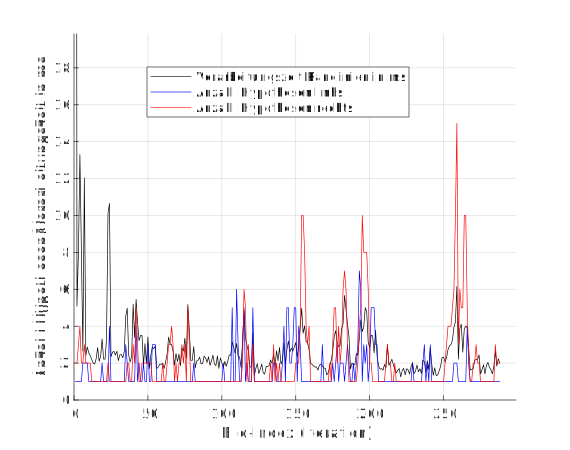
\includegraphics[width=0.6\textwidth]{evaluation_riverflow_hypos_times_04}
\caption{Zusammenhang Anzahl verfolgter Hypothesen \&\ Dauer der Detektion seitlicher Fahrbahnmarkierungen; \SI{4}{cm} Abstand Quader zu Fahrspur}
\label{evaluation:riverflow:hypos:times_04}
\end{figure}

\subsection{Objekte in der Gegenspur}
Da, bedingt durch die Verifikation, erkannte Fahrbahnmarkierungen nur in die Karte eingetragen werden, wenn sie zu mindestens einer weiteren erkannten Linie passen, muss für eine Fehlerkennung diese Bedingung auch durch die platzierten \glqq Störobjekte\grqq\ erfüllt werden. Da sich das Fahrzeug nur auf der rechten Straßenseite fortbewegt, wurde der Versuchsaufbau in Abb. \ref{fig:evaluation:riverflow:test_kontraste_versuchsaufbau_baustelle} gewählt, welcher diesem Kriterium nachkommt.
\begin{figure}[htbp] % [htb]
\centering
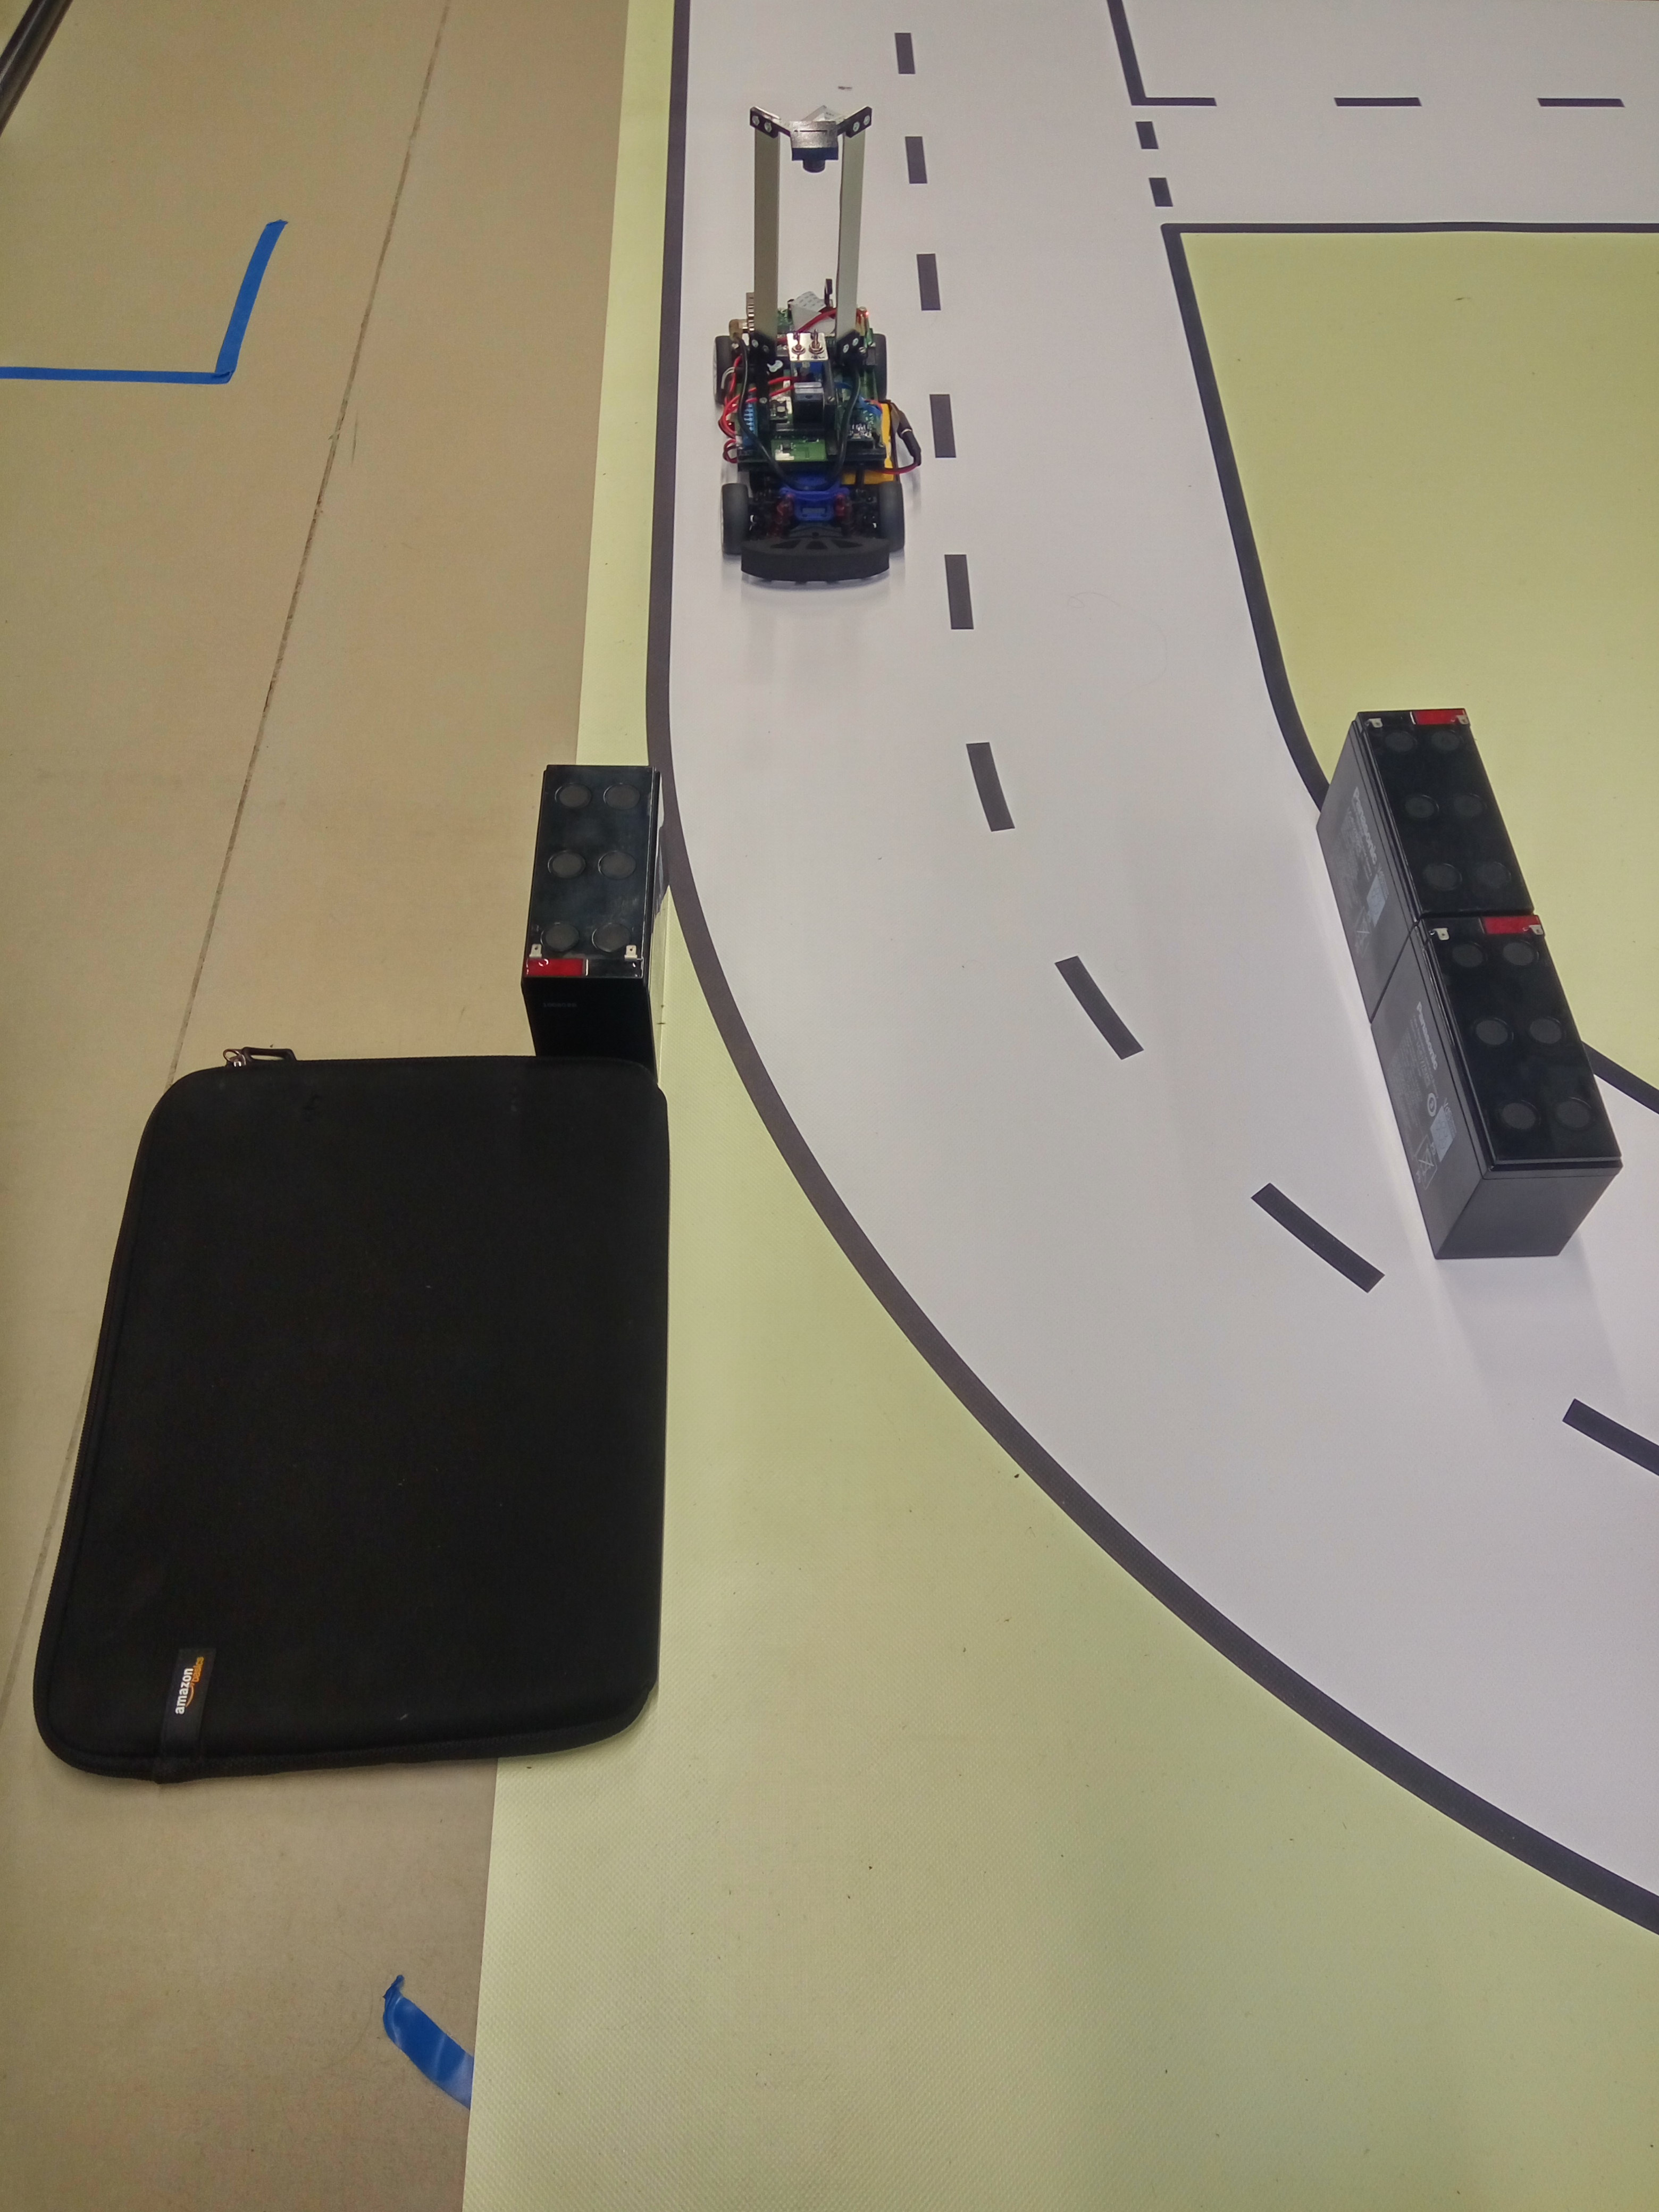
\includegraphics[width=0.5\textwidth]{evaluation_riverflow_test_kontraste_versuchsaufbau_baustelle}
\caption{Versuchsaufbau mit \glqq Störobjekt\grqq\ auf der Gegenfahrspur}
\label{fig:evaluation:riverflow:test_kontraste_versuchsaufbau_baustelle}
\end{figure}

Die Fehldetektion der linken Fahrbahnmarkierung konnte somit provoziert werden. Da die richtig erkannte rechte Randlinie jedoch mehr Punkte generierte und anhand der Mittellinie verifiziert wurde, sind diese zwei Linien noch korrekt in die Weltkarte eingetragen (s. Abb. \ref{fig:evaluation:riverflow:baustelle_weltkarte_1} und \ref{fig:evaluation:riverflow:baustelle_riverflow_plot_1}). Das Modellauto fuhr ein wenig rechts der Ideallinie, kam aber nicht stark vom Kurs ab.
Erst durch Abdecken der Mittellinie (s. Abb. \ref{fig:evaluation:riverflow:baustelle_weltkarte_2} und \ref{fig:evaluation:riverflow:baustelle_riverflow_plot_2}) und die somit fehlende Validierungsmöglichkeit der richtig erkannten rechten Fahrbahnmarkierung konnte der Roboter vom Kurs abgebracht werden und verließ die Straße völlig.
\begin{figure}[htbp] % [htb]
%\centering
%\hfill
\subfloat[Einzelbild mit Mittellinie \label{fig:evaluation:riverflow:baustelle_riverflow_plot_1}]{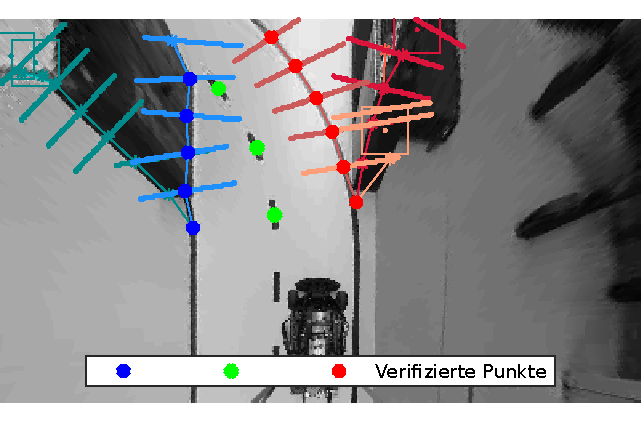
\includegraphics[width=0.49\textwidth]{evaluation_riverflow_baustelle_riverflow_plot_1}}
\hfill
\subfloat[Einzelbild ohne Mittellinie\label{fig:evaluation:riverflow:baustelle_riverflow_plot_2}]{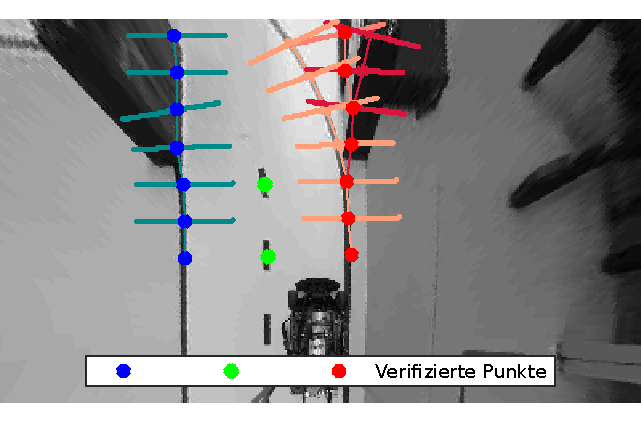
\includegraphics[width=0.49\textwidth]{evaluation_riverflow_baustelle_riverflow_plot_2}}
\hfill
\subfloat[Weltkarte mit Mittellinie\label{fig:evaluation:riverflow:baustelle_weltkarte_1}]{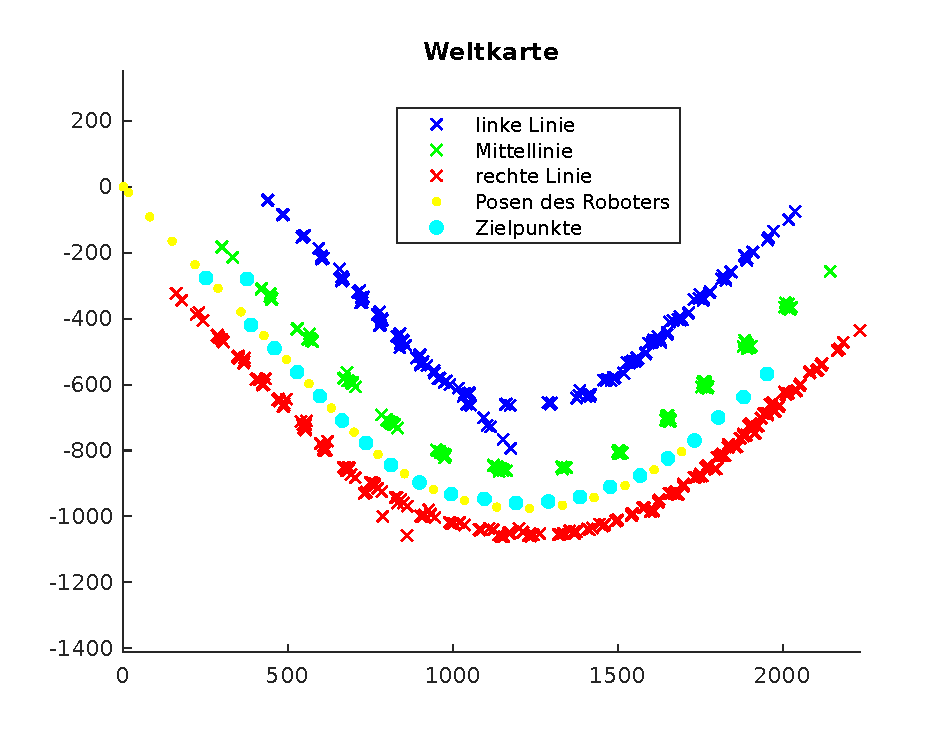
\includegraphics[scale=\mtlstscale]{evaluation_riverflow_baustelle_weltkarte_1}}
\hfill
\subfloat[Weltkarte ohne Mittellinie\label{fig:evaluation:riverflow:baustelle_weltkarte_2}]{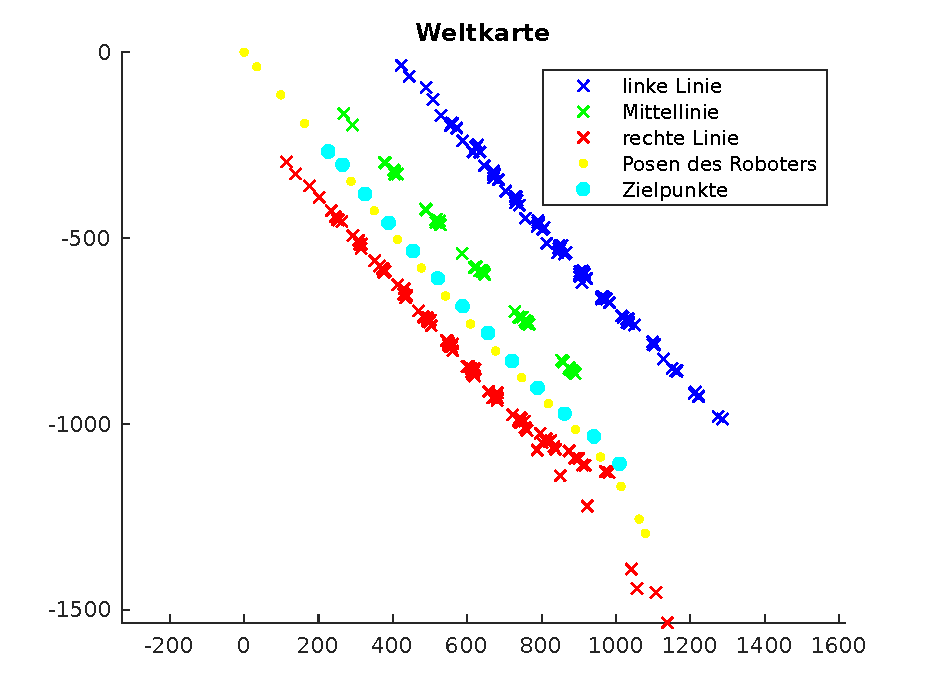
\includegraphics[scale=\mtlstscale]{evaluation_riverflow_baustelle_weltkarte_2}}
%\hfill
\caption{Versuch mit \glqq Störobjekt\grqq\ auf der Gegenfahrspur}
\label{fig:evaluation:riverflow:baustelle}
\end{figure}
